\section{Progettazione piattaforma}
%a partire dal git in automatico su ckan con metadati
%\begin{quoting}
Con delibera 14 del 19/01/2012 il Comune di Vigevano, nell'ambito del Progetto InnoVi, cofinanziato dalla regione, ha adottato, in riuso dal Comune di Milano, la piattaforma \textbf{GIT}, un integratore di banche dati interne ed esterne all'ente e relativa cartografia, con il project management di Ancitel Lombardia ed il supporto tecnico della societ� HiWeb Srl della Regione Umbria che ha contribuito a far nascere e crescere tale sistema.
%[...]
Il sistema GIT � un ricco contenitore di informazioni alfanumeriche e grafiche correlate, periodicamente aggiornate, e che, per questo, � un candidato naturale ad alimentare dei dataset di dati da rendere disponibili con licenze open, opportunamente filtrati ed aggregati allo scopo di tutelare la privacy.
\cite{CittaVigevano-GCn104}
%\end{quoting}
Vogliamo quindi una piattaforma che permetta di integrare le informazioni presenti sulla piattaforma GIT con il portale Open Data che verr� realizzato.
Per fare ci� sono percorribili tre strade distinte:
\begin{enumerate}
\item Effettuare periodicamente delle esportazioni dei dati da GIT per caricarle sulla piattaforma.
\item Effettuare l'aggiornamento dei dati sulla piattaforma ogni volta che vengono aggiornati su GIT in automatico.
\item Permettere alla piattaforma di accedere direttamente ai dati di GIT.
\end{enumerate}

La terza soluzione presenta dei problemi di sicurezza, perch� per realizzarla bisogna modificare GIT creando un interfaccia che permetta l'interrogazione ai dati dall'esterno. Ci� pu� diventare un problema nel momento in cui si creano delle API di interrogazioni generiche e quindi in alcune occasioni si finisce a violare la privacy degli utenti.

La prima soluzione pu� essere applicata nei casi in cui le informazioni hanno una frequenza di aggiornamento rada, ma diventa impraticabile nel momento in cui i dati vengo aggiornati con una frequenza rilevante, in quando bisogna fare manualmente un aggiornamento ogni volta.

La soluzione vincente risulta quindi essere la seconda, essa comporta un controllo degli eventi sulla piattaforma GIT e l'esistenza di un sistema di aggiornamento automatizzato (senza intervento umano) sulla piattaforma Open Data.
Nell'ottica del riutilizzo del software, questa componente deve essere in grandi di controllare eventuali aggiornamenti di GIT, di anonimizzare i dati e di inserirli nella piattaforma attraverso API.\\

%Catalogo e dizionario
Al fine di agevolare l'integrazione tra la piattaforma e applicazioni di terze parti si vuole rendere disponibile un \textbf{catalogo} contenente tutti i dataset e i relativi metadati. Con Metadati si intendono le informazioni riguardanti il singolo dataset quali il suo nome, la sua descrizione, il formato del file, la sua data di ultima modifica, il link a cui raggiungere la risorsa, ...

Si vuole inoltre rendere disponibile per ogni dataset il dizionario dei dati in esso contenuto. Ci� vuol dire che nel catalogo sar� presente anche l'informazione della tabella per ogni singolo dataset.

In questo modo � possibile interrogare il dataset sapendo a priori il tipo di dato che � contenuto in esso.\\

%Triggher e workflow
Si � scelto di utilizzare una piattaforma open source in accordo con il Comune di Vigevano e di conseguenza CKAN � stata la piattaforma sulla quale si � scelto di implementare i requisiti.
Al fine di rendere compatibile le modifiche apportate alla piattaforma CKAN tra le varie versioni della stessa si � deciso di analizzarlo come una �scatola nera�, senza mettere mano al codice sorgente di CKAN.

\begin{figure}[htbp]
   \centering
   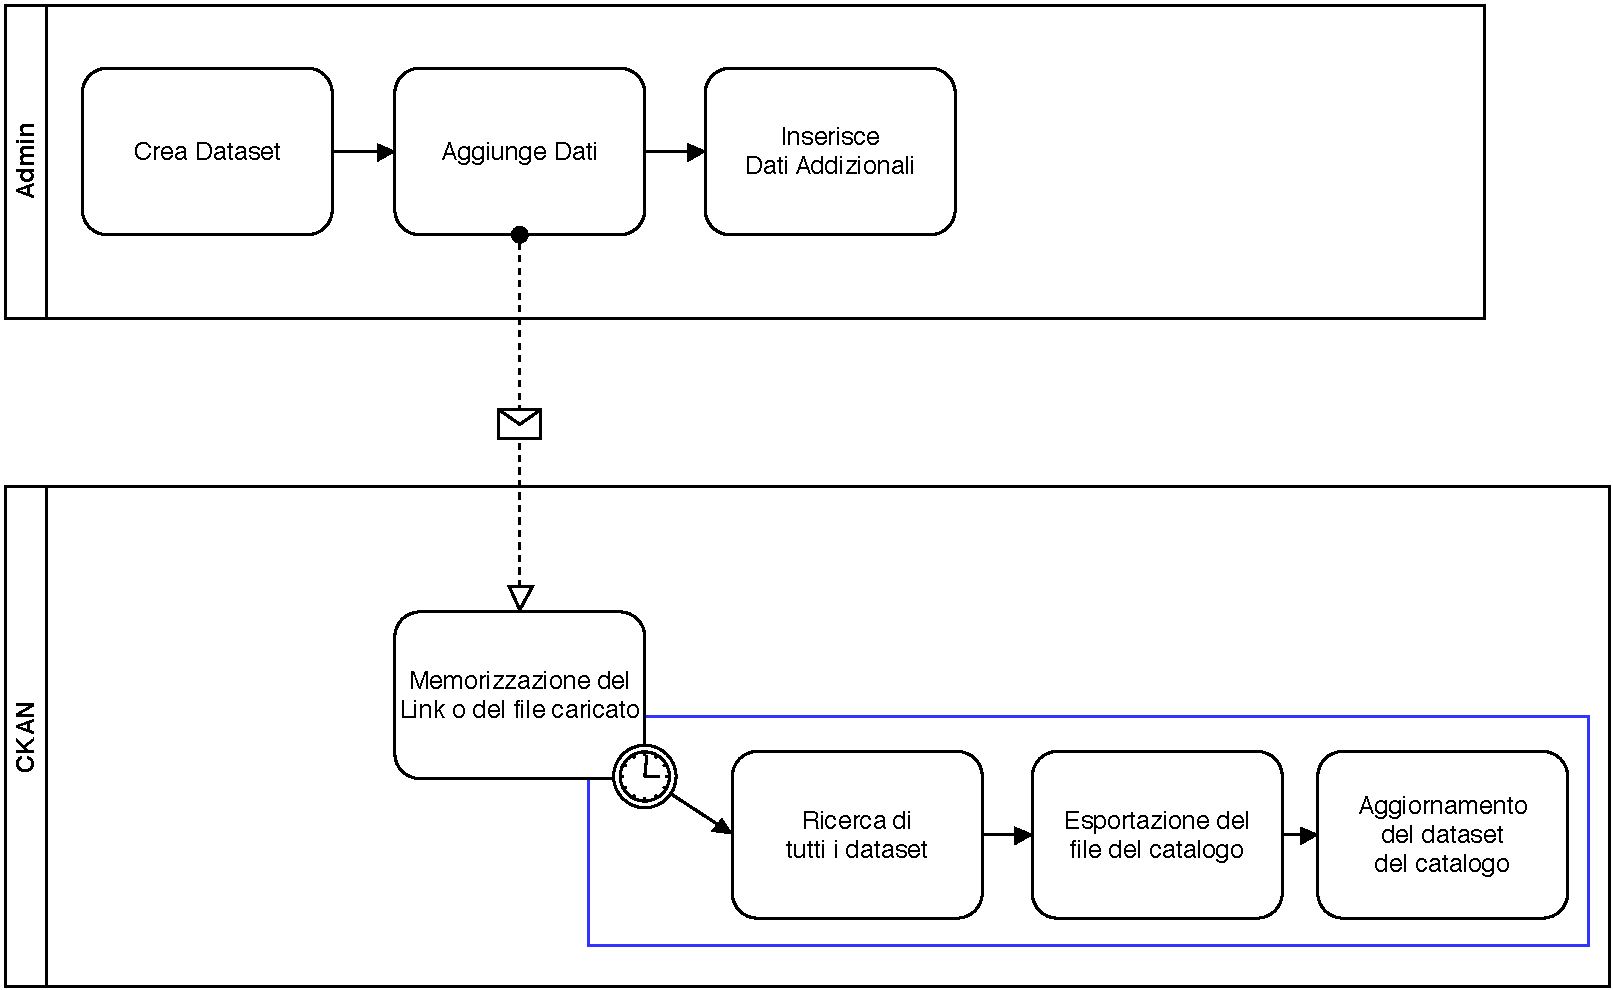
\includegraphics[scale=0.5]{img/workflow-creazione-dataset} % requires the graphicx package
   \caption{Workflow dell�aggiornamento del catalogo al momento dell�inserimento di un nuovo dataset}
   \label{fig:workflow}
\end{figure}

La progettazione del catalogo � quindi stata fatta come mostrato in fig. \ref{fig:workflow} inserendo un triggher (una procedura che viene eseguita in maniera automatica in coincidenza di un determinato evento) che ad ogni aggiornamento nel database della tabella contenente i dataset venga fatta una query che restituisce il catalogo (facendo un join tra diverse tabelle) e la esporti in formato CSV. Il file contenete il catalogo � esso stesso parte integrante della piattaforma essendo a sua volta un dataset.
